\section{Date: 2026-07-27}
\noindent \textbf{Series ID: WUPINZL} 

\noindent This series is titled World Pandemic Uncertainty Index for New Zealand and has a frequency of Quarterly. The units are Index and the seasonal adjustment is Not Seasonally Adjusted.The observation start date is 1996-01-01 and the observation end date is 2026-01-01.The popularity of this series is 1. \\ 

\noindent \textbf{Series ID: PRCMUCON} 

\noindent This series is titled Total Private Construction Spending: Communication in the United States and has a frequency of Monthly. The units are Millions of Dollars and the seasonal adjustment is Not Seasonally Adjusted.The observation start date is 1993-01-01 and the observation end date is 2026-05-01.The popularity of this series is 1. \\ 

\subsection{Raw Regression}
\noindent Regresses the two series against each other directly. A significant result here can come just as easily from both series sharing a long-run trend as from any real relationship.

\begin{center}
\begin{tabular}{lclc}
\toprule
\textbf{Dep. Variable:}       & value\_fred\_PRCMUCON & \textbf{  R-squared:         } &     0.008   \\
\textbf{Model:}               &          OLS          & \textbf{  Adj. R-squared:    } &    -0.000   \\
\textbf{Method:}              &     Least Squares     & \textbf{  F-statistic:       } &    0.9862   \\
\textbf{Date:}                &    Mon, 27 Jul 2026   & \textbf{  Prob (F-statistic):} &    0.323    \\
\textbf{Time:}                &        14:06:59       & \textbf{  Log-Likelihood:    } &   -897.76   \\
\textbf{No. Observations:}    &            121        & \textbf{  AIC:               } &     1800.   \\
\textbf{Df Residuals:}        &            119        & \textbf{  BIC:               } &     1805.   \\
\textbf{Df Model:}            &              1        & \textbf{                     } &             \\
\textbf{Covariance Type:}     &       nonrobust       & \textbf{                     } &             \\
\bottomrule
\end{tabular}
\begin{tabular}{lcccccc}
                              & \textbf{coef} & \textbf{std err} & \textbf{t} & \textbf{P$> |$t$|$} & \textbf{[0.025} & \textbf{0.975]}  \\
\midrule
\textbf{const}                &    1632.8538  &       37.497     &    43.547  &         0.000        &     1558.607    &     1707.101     \\
\textbf{value\_fred\_WUPINZL} &      10.4150  &       10.487     &     0.993  &         0.323        &      -10.351    &       31.181     \\
\bottomrule
\end{tabular}
\begin{tabular}{lclc}
\textbf{Omnibus:}       &  3.754 & \textbf{  Durbin-Watson:     } &    0.365  \\
\textbf{Prob(Omnibus):} &  0.153 & \textbf{  Jarque-Bera (JB):  } &    2.215  \\
\textbf{Skew:}          &  0.059 & \textbf{  Prob(JB):          } &    0.330  \\
\textbf{Kurtosis:}      &  2.348 & \textbf{  Cond. No.          } &     3.63  \\
\bottomrule
\end{tabular}
%\caption{OLS Regression Results}
\end{center}

Notes: \newline
 [1] Standard Errors assume that the covariance matrix of the errors is correctly specified.

\begin{figure}
\centering
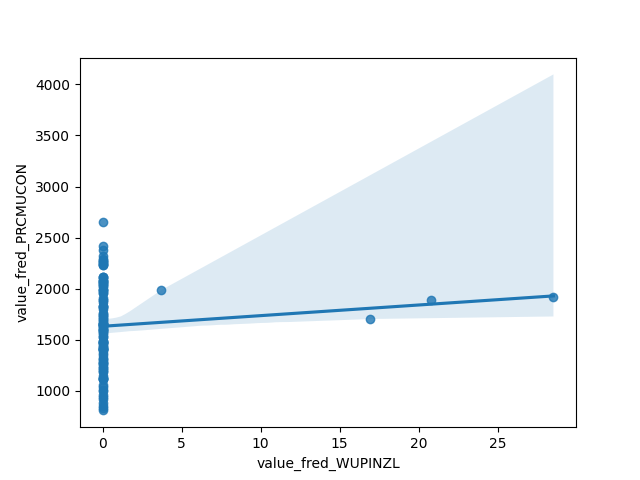
\includegraphics[scale = 0.9]{plots/plot_2026-07-27.png}
\caption{Raw Regression Plot for 2026-07-27}
\end{figure}
\newpage
\subsection{Detrended Regression}
\noindent Regresses the residuals of each series after removing its own linear time trend, so a shared trend can no longer drive the result on its own. A relationship that stays significant here is better evidence of a genuine link between the two series.

\begin{center}
\begin{tabular}{lclc}
\toprule
\textbf{Dep. Variable:}                  & value\_fred\_PRCMUCON\_detrended & \textbf{  R-squared:         } &     0.005   \\
\textbf{Model:}                          &               OLS                & \textbf{  Adj. R-squared:    } &    -0.004   \\
\textbf{Method:}                         &          Least Squares           & \textbf{  F-statistic:       } &    0.5697   \\
\textbf{Date:}                           &         Mon, 27 Jul 2026         & \textbf{  Prob (F-statistic):} &    0.452    \\
\textbf{Time:}                           &             14:06:59             & \textbf{  Log-Likelihood:    } &   -858.73   \\
\textbf{No. Observations:}               &                 121              & \textbf{  AIC:               } &     1721.   \\
\textbf{Df Residuals:}                   &                 119              & \textbf{  BIC:               } &     1727.   \\
\textbf{Df Model:}                       &                   1              & \textbf{                     } &             \\
\textbf{Covariance Type:}                &            nonrobust             & \textbf{                     } &             \\
\bottomrule
\end{tabular}
\begin{tabular}{lcccccc}
                                         & \textbf{coef} & \textbf{std err} & \textbf{t} & \textbf{P$> |$t$|$} & \textbf{[0.025} & \textbf{0.975]}  \\
\midrule
\textbf{const}                           &    1.119e-11  &       26.801     &  4.17e-13  &         1.000        &      -53.069    &       53.069     \\
\textbf{value\_fred\_WUPINZL\_detrended} &      -5.8542  &        7.756     &    -0.755  &         0.452        &      -21.212    &        9.503     \\
\bottomrule
\end{tabular}
\begin{tabular}{lclc}
\textbf{Omnibus:}       & 14.526 & \textbf{  Durbin-Watson:     } &    0.687  \\
\textbf{Prob(Omnibus):} &  0.001 & \textbf{  Jarque-Bera (JB):  } &   17.629  \\
\textbf{Skew:}          &  0.701 & \textbf{  Prob(JB):          } & 0.000149  \\
\textbf{Kurtosis:}      &  4.238 & \textbf{  Cond. No.          } &     3.46  \\
\bottomrule
\end{tabular}
%\caption{OLS Regression Results}
\end{center}

Notes: \newline
 [1] Standard Errors assume that the covariance matrix of the errors is correctly specified.

\begin{figure}
\centering
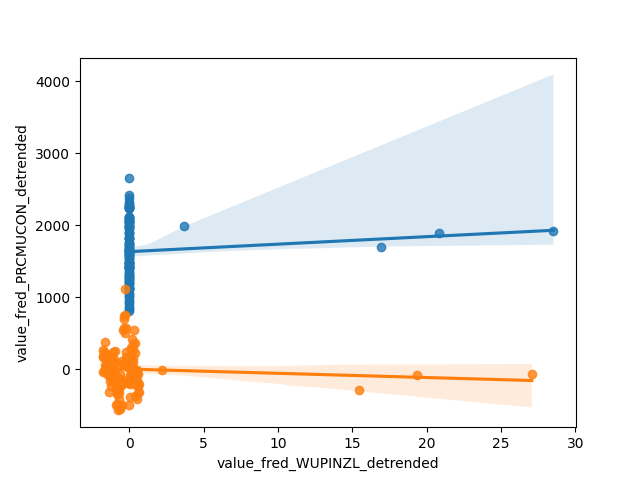
\includegraphics[scale = 0.9]{plots/plot_2026-07-27_detrended.png}
\caption{Detrended Regression Plot for 2026-07-27}
\end{figure}
\newpage
